% Options for packages loaded elsewhere
\PassOptionsToPackage{unicode}{hyperref}
\PassOptionsToPackage{hyphens}{url}
\documentclass[
  ignorenonframetext,
]{beamer}
\newif\ifbibliography
\usepackage{pgfpages}
\setbeamertemplate{caption}[numbered]
\setbeamertemplate{caption label separator}{: }
\setbeamercolor{caption name}{fg=normal text.fg}
\beamertemplatenavigationsymbolsempty
% remove section numbering
\setbeamertemplate{part page}{
  \centering
  \begin{beamercolorbox}[sep=16pt,center]{part title}
    \usebeamerfont{part title}\insertpart\par
  \end{beamercolorbox}
}
\setbeamertemplate{section page}{
  \centering
  \begin{beamercolorbox}[sep=12pt,center]{section title}
    \usebeamerfont{section title}\insertsection\par
  \end{beamercolorbox}
}
\setbeamertemplate{subsection page}{
  \centering
  \begin{beamercolorbox}[sep=8pt,center]{subsection title}
    \usebeamerfont{subsection title}\insertsubsection\par
  \end{beamercolorbox}
}
% Prevent slide breaks in the middle of a paragraph
\widowpenalties 1 10000
\raggedbottom
\AtBeginPart{
  \frame{\partpage}
}
\AtBeginSection{
  \ifbibliography
  \else
    \frame{\sectionpage}
  \fi
}
\AtBeginSubsection{
  \frame{\subsectionpage}
}
\usepackage{iftex}
\ifPDFTeX
  \usepackage[T1]{fontenc}
  \usepackage[utf8]{inputenc}
  \usepackage{textcomp} % provide euro and other symbols
\else % if luatex or xetex
  \usepackage{unicode-math} % this also loads fontspec
  \defaultfontfeatures{Scale=MatchLowercase}
  \defaultfontfeatures[\rmfamily]{Ligatures=TeX,Scale=1}
\fi
\usepackage{lmodern}
\ifPDFTeX\else
  % xetex/luatex font selection
\fi
% Use upquote if available, for straight quotes in verbatim environments
\IfFileExists{upquote.sty}{\usepackage{upquote}}{}
\IfFileExists{microtype.sty}{% use microtype if available
  \usepackage[]{microtype}
  \UseMicrotypeSet[protrusion]{basicmath} % disable protrusion for tt fonts
}{}
\makeatletter
\@ifundefined{KOMAClassName}{% if non-KOMA class
  \IfFileExists{parskip.sty}{%
    \usepackage{parskip}
  }{% else
    \setlength{\parindent}{0pt}
    \setlength{\parskip}{6pt plus 2pt minus 1pt}}
}{% if KOMA class
  \KOMAoptions{parskip=half}}
\makeatother
\usepackage{graphicx}
\makeatletter
\newsavebox\pandoc@box
\newcommand*\pandocbounded[1]{% scales image to fit in text height/width
  \sbox\pandoc@box{#1}%
  \Gscale@div\@tempa{\textheight}{\dimexpr\ht\pandoc@box+\dp\pandoc@box\relax}%
  \Gscale@div\@tempb{\linewidth}{\wd\pandoc@box}%
  \ifdim\@tempb\p@<\@tempa\p@\let\@tempa\@tempb\fi% select the smaller of both
  \ifdim\@tempa\p@<\p@\scalebox{\@tempa}{\usebox\pandoc@box}%
  \else\usebox{\pandoc@box}%
  \fi%
}
% Set default figure placement to htbp
\def\fps@figure{htbp}
\makeatother
\setlength{\emergencystretch}{3em} % prevent overfull lines
\providecommand{\tightlist}{%
  \setlength{\itemsep}{0pt}\setlength{\parskip}{0pt}}
% Slide layout defaults for warning-clean scientific decks.
\usepackage{etoolbox}
\IfFileExists{xurl.sty}{\usepackage{xurl}}{}
\IfFileExists{seqsplit.sty}{\usepackage{seqsplit}}{\newcommand{\seqsplit}[1]{#1}}
\protected\def\breakseq#1{\seqsplit{#1}}
\protected\def\breaktt#1{\begingroup\ttfamily\seqsplit{#1}\endgroup}
\setlength{\emergencystretch}{6em}
\tolerance=5000
\hbadness=10000
\hfuzz=1pt
\setlength{\tabcolsep}{2pt}
\AtBeginEnvironment{longtable}{\tiny\renewcommand{\arraystretch}{0.86}\setlength{\tabcolsep}{1pt}}
\AtBeginEnvironment{tabular}{\tiny\renewcommand{\arraystretch}{0.86}\setlength{\tabcolsep}{1pt}}

% Natbib and cross-reference fallbacks — slides don't load natbib
% or cleveref, but combined-PDF manuscript prose may emit these
% commands. The fallback renders citations as a bracketed key list
% and cross-references as detokenized labels so slides don't fail on
% undefined control sequences or raw underscores. \providecommand is
% a no-op if packages load later.
\providecommand{\citep}[1]{[#1]}
\providecommand{\citet}[1]{#1}
\providecommand{\citealp}[1]{#1}
\providecommand{\citeauthor}[1]{#1}
\providecommand{\citeyear}[1]{#1}
\providecommand{\cref}[1]{\texttt{\detokenize{#1}}}
\providecommand{\Cref}[1]{\texttt{\detokenize{#1}}}

\newtheorem{proposition}{Proposition}
\newtheorem{hypothesis}{Hypothesis}
\usepackage{bookmark}
\IfFileExists{xurl.sty}{\usepackage{xurl}}{} % add URL line breaks if available
\urlstyle{same}
% fallback for those not using the hyperref driver hyperxmp:
\makeatletter
\@ifundefined{xmpquote}{\newcommand{\xmpquote}[1]{#1}}{}
\makeatother
\hypersetup{
  hidelinks,
  pdfcreator={LaTeX via pandoc}}

\author{\texorpdfstring{}{}}
\date{}

\begin{document}

\section{Integrative Model: The Human-Human DigiPPPiP
Kernel}\label{sec:integrative}

\begin{frame}[fragile,allowframebreaks]{Integrative Model: The
Human-Human DigiPPPiP Kernel}
DigiPPPiP can be summarized as a cyberphysical relational practice. Its
first layer is a coupled modeling lens: partners can be described as
updating expectations about each other's intentions through shared
marks, with the formal primitive isolated in
\breakseq{[@sec:formalisms\_appendix]}. Its second layer is
cyber-phenomenological co-presence: marks carry embodied gesture across
physical, digital, and hybrid surfaces. Its third layer is narrative
information architecture: sessions become symbolic trajectories with
entropy, surprise, and convergence.

The fourth layer is neuroergonomic design: the interface should preserve
attention, reduce technoference, and support flow. The fifth layer is
place-relational grounding: sessions can bind two bodies, two
environments, and one artifact. The sixth layer is accessibility: input
and feedback should adapt to participants rather than forcing
participants to adapt to one canonical interface. The word
``accessibility'' is used here as a design and validation program, not
as a universal guarantee.

The seventh layer is temporal flexibility. Synchronous, semisynchronous,
and asynchronous modes are not rank-ordered; they answer different
relational constraints. The eighth layer is measurement.
Active-inference, narrative-information, event-log, accessibility,
outcome-model, and geometric-hyperscanning tools give the framework
empirical handles without letting the manuscript pretend that conceptual
simulations are evidence.

The model can also be collapsed to a minimum viable DigiPPPiP loop:
partner acts, mark persists, other partner perceives, response changes
the shared field, and both partners retain agency over what remains.
Every larger layer should be justified by how it strengthens that loop.
If a feature does not improve perception, action, persistence,
interpretation, access, or consent, it is outside the core framework
even if it is technically impressive. The architecture in
\breakseq{[@fig:cpss\_architecture]} operationalizes that rule by separating
the kernel from instrumentation, modeling, optional AI support, and
publication governance.

The systems-governance layer makes that collapse enforceable.
\breaktt{src/systems\_governance.py} treats the human-human mark loop as
the kernel and places event logs, place context, optional physiology, AI
assistance, and clinical translation in named boundary positions. This
matters because a system boundary is a design decision, not a discovered
fact: moving physiology, AI, or clinical translation into the kernel
would change the participant contract and the evidence burden. The
integrative model therefore remains reversible. Branches can be removed,
disabled, coarsened, or downgraded without losing the core practice.

\breakseq{[@fig:framework\_template]} summarizes the reusable visual grammar
that holds these layers together. Actors, artifacts, signals, contexts,
diagnostics, and evidence maps are styled consistently so captions can
identify what is encoded, which generator produced it, what claim
strength it supports, and what caveat remains. The grammar now has a
stronger architecture role: human actions, optional AI branches,
computed diagnostics, and publication artifacts should be visually
separable even when they appear in one system figure.

\begin{figure}
\centering
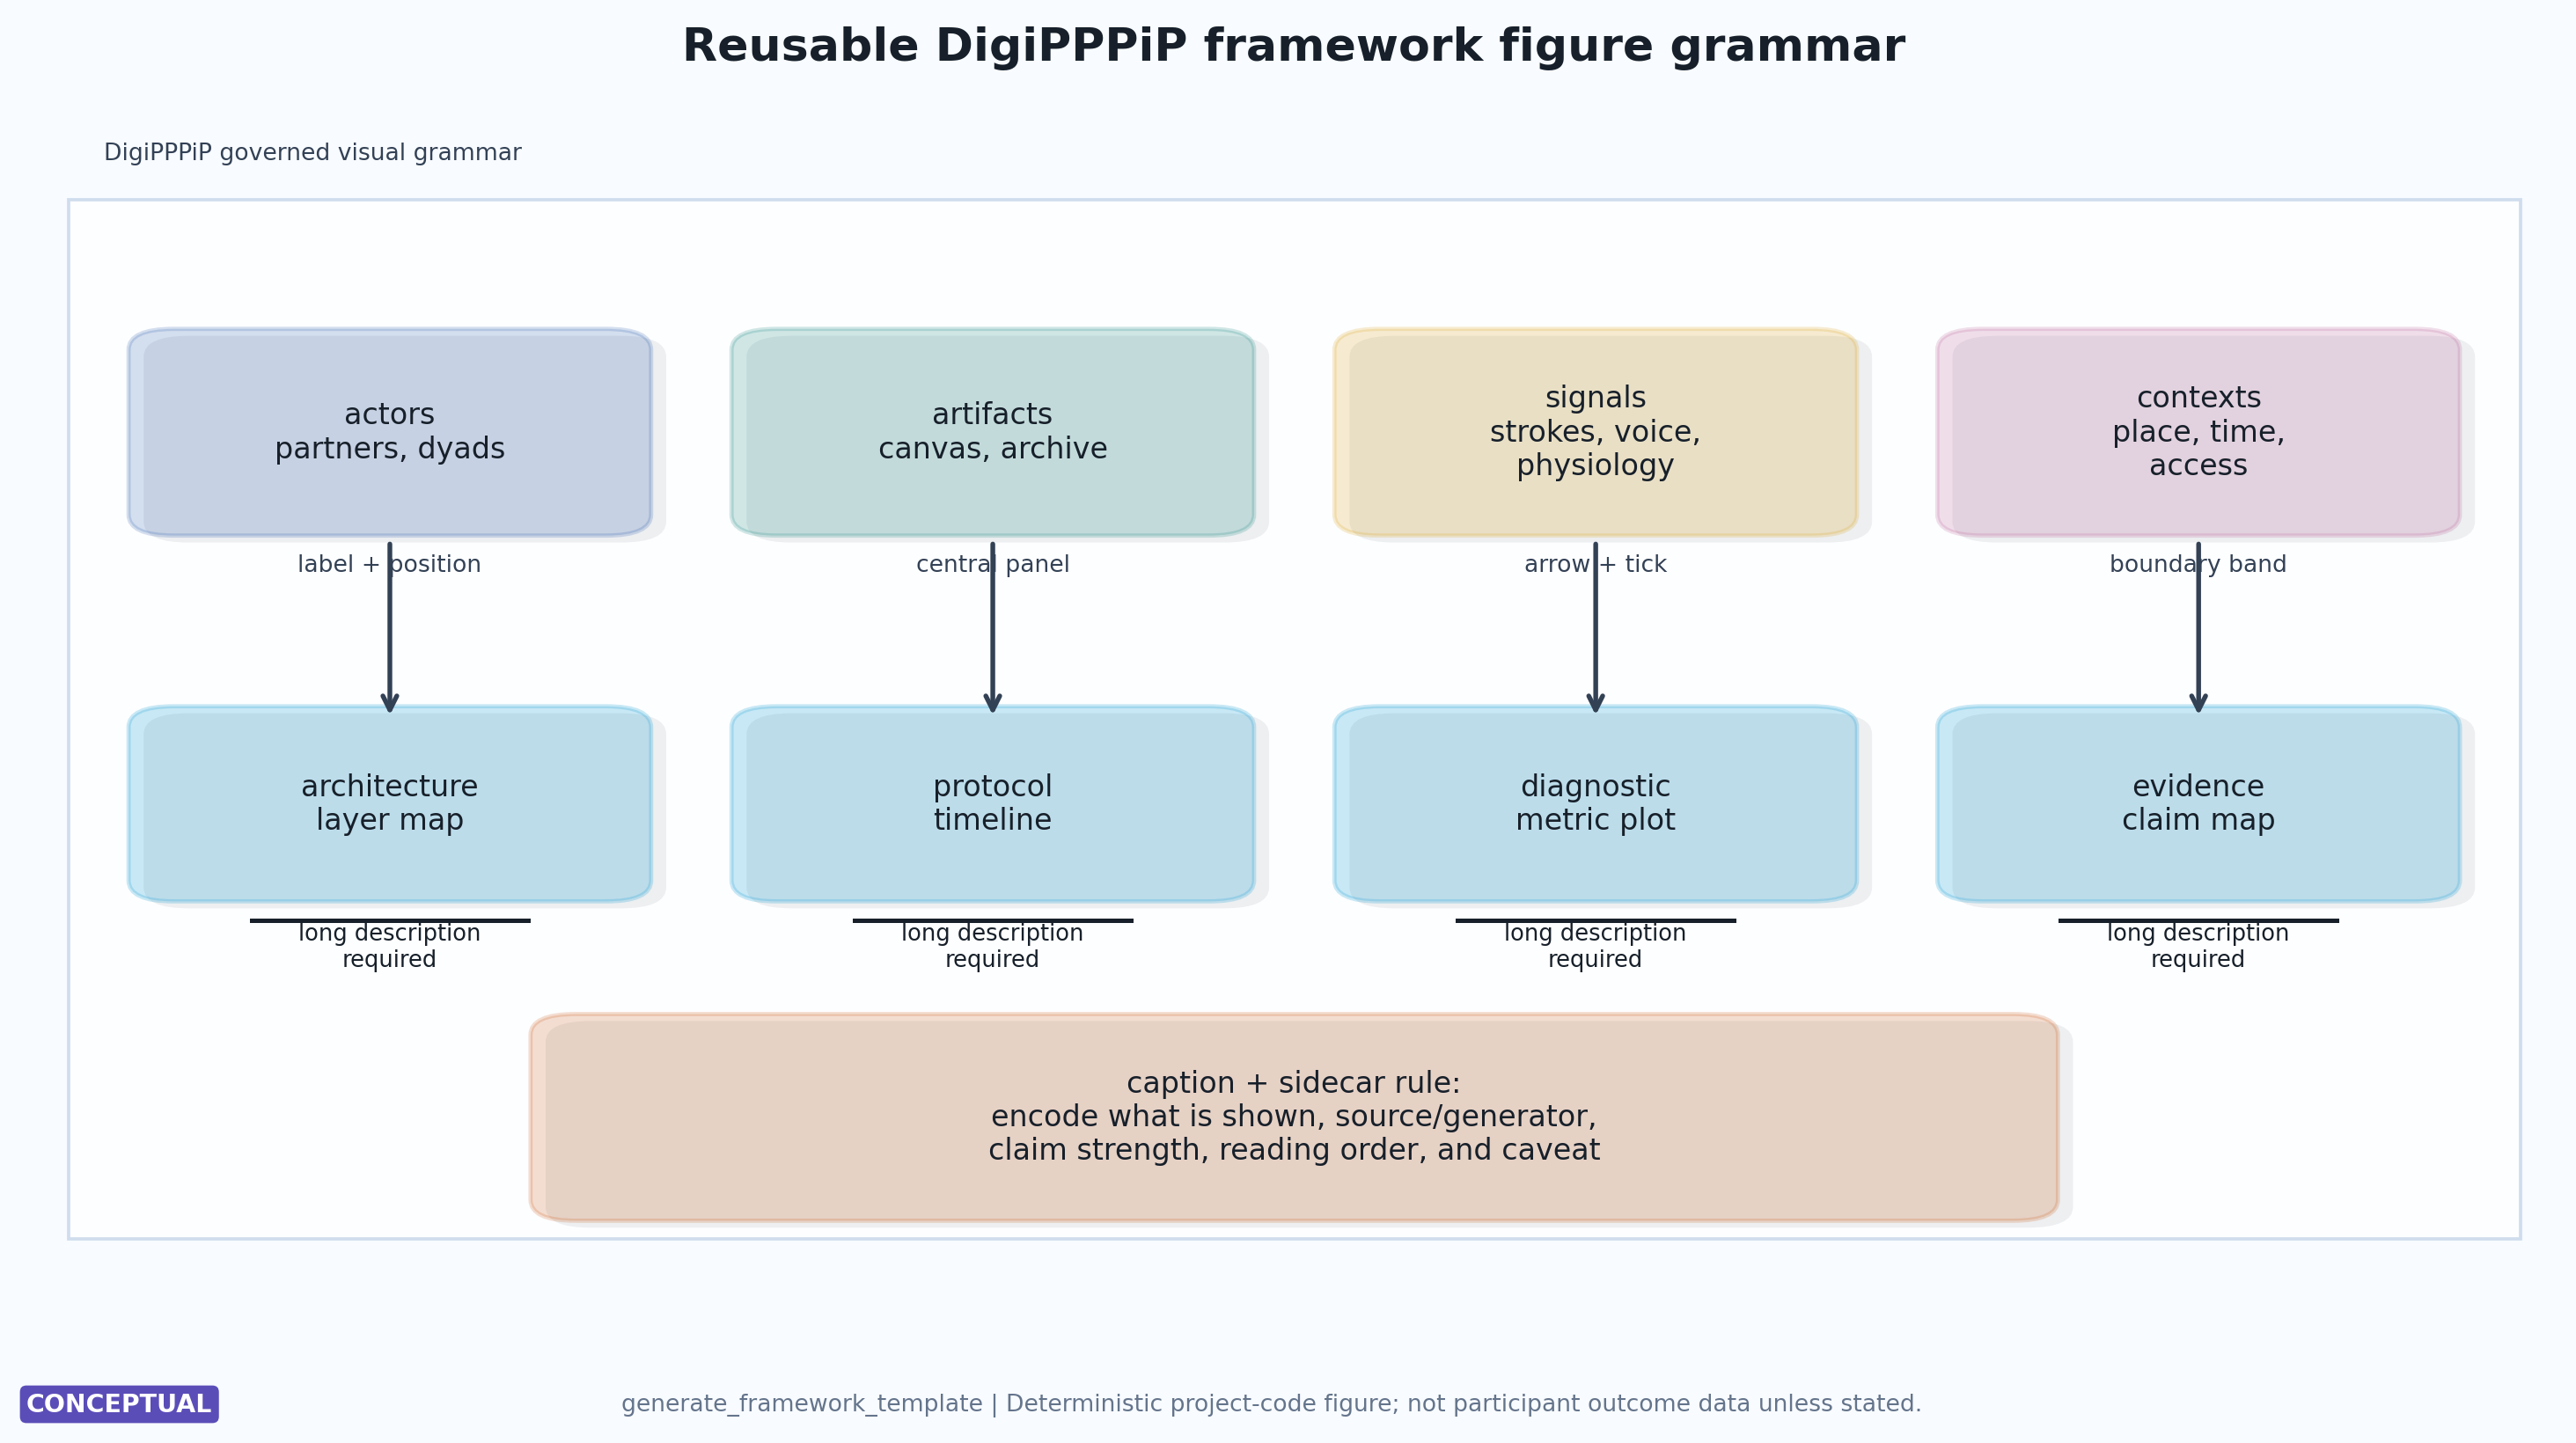
\includegraphics[width=0.9\linewidth,height=0.46\textheight,keepaspectratio,alt={Reusable DigiPPPiP figure grammar for actors, artifacts, signals, contexts, architecture maps, protocol timelines, diagnostic plots, and evidence maps. The figure is generated by generate\_framework\_template(); read the upper row as semantic roles, the small labels as non-color channels, the middle row as reusable figure forms, and the lower box as the caption and long-description rule applied throughout the manuscript. It supports integrative consistency, not empirical validation, and future data figures should keep the same claim-boundary discipline.}]{../figures/framework_template.png}
\caption{Reusable DigiPPPiP figure grammar for actors, artifacts,
signals, contexts, architecture maps, protocol timelines, diagnostic
plots, and evidence maps. The figure is generated by
\protect\breaktt{generate\_framework\_template()}; read the upper row as
semantic roles, the small labels as non-color channels, the middle row
as reusable figure forms, and the lower box as the caption and
long-description rule applied throughout the manuscript. It supports
integrative consistency, not empirical validation, and future data
figures should keep the same claim-boundary
discipline.}\label{fig:framework_template}
\end{figure}
\end{frame}

\end{document}
